\documentclass[a4paper,12pt]{article}
\usepackage[left=30mm,right=20mm, top=20mm,bottom=20mm,bindingoffset=0cm]{geometry}
\usepackage{style}
\usepackage{tikz-cd}
% \usepackage[12pt]{extsizes}
\usepackage{cite}
\usepackage{color}
\usepackage{xcolor}
\newcommand{\TODO}[1]{{\color{magenta}#1}}
\usepackage{hyperref}
\usepackage{pdfpages}

\hypersetup{
	colorlinks   = true, %Colours links instead of ugly boxes
	urlcolor     = blue, %Colour for external hyperlinks
	linkcolor    = blue, %Colour of internal links
	citecolor    = red %Colour of citations
}

\newcommand{\Href}[2]{\hyperref[#2]{#1~\ref{#2}}}

% \relpenalty=10000
% \binoppenalty=10000

\def\int{\mathop{\rm int}}
\def\vol{\mathop{\rm vol}}
\def\co{\mathop{\rm conv}}
\def\rk{\mathop{\rm rk}}
\def\span{\mathop{\rm span}}
\def\diag{\mathop{\rm diag}}
\def\Gr{\mathbf{\rm Gr}}
\def\low{\text{\rm L\"ow}}
\def\john{\mathbf{\rm John}}

\def\changemargin#1#2{\list{}{\rightmargin#2\leftmargin#1}\item[]}
\let\endchangemargin=\endlist 

% \renewcommand{\proofname}{\textbf{Доказательство}}


\newcommand{\cube}{\square}
\newcommand{\crosp}{\Diamond}
\newcommand{\bigzero}{\makebox(0,0){\text{\huge0}}}
\newcommand{\HRule}{\rule{\linewidth}{0.5mm}}
\newcommand{\comm}[1]{\textcolor{red}{#1} }
\newcommand{\lb}[1]{#1\nobreak\discretionary{}{\hbox{\ensuremath{#1}}}{}}

\linespread{1.5}
 
\newtheorem{lem}{Лемма}[section]
\newtheorem{prop}{Утверждение}[section]
\newtheorem{theorem}{Теорема}[section]
\newtheorem{cor}{Следствие}[section]

% \theoremstyle{definition}
\newtheorem*{defin*}{Определение}
% \newtheorem{rem}[defin*]{Замечание}
% \newtheorem{exl}[defin*]{Пример}

\numberwithin{equation}{section}

\begin{document}

	% \includepdf{title/title.pdf}
	\tableofcontents
	\newpage

	\section{Введение}
	\textit{Кросс-политоп} $\crosp^n$, или гипероктаэдр, --- это выпуклый центрально-симметричный многогранник, являющийся выпуклой оболочкой векторов стандартного базиса $\RR^n$ и противоположных к ним векторов. Эквивалентно, это единичный шар в $\ell_1$-норме.
	\begin{figure}[h!]
		\begin{center}
		\includegraphics[scale=0.5]{pics/crosp.pdf}
		\caption{2- и 3-мерный кросс-политоп}
		\end{center}
	\end{figure}

	Известно, что всякий выпуклый центрально-симметричный многогранник в $\RR^n$ аффинно эквивалентен проекции кросс-политопа большей размерности на $\RR^n$, поэтому проекции кросс-политопа удобно рассматривать как некоторое стандартное положение выпуклых центрально-симметричных многогранников. Вследствие этого вопросы оценки объёмов многогранников естественно связаны с объёмами проекций кросс-политопов.

	Нас интересует поиск необходимых условий, при которых объём ортогональной проекции $n$-мерного кросс-политопа на $k$-мерное подпространство $H_k\subset\RR^n$ достигает максимума. Иными словами, мы исследуем на максимум функцию
		\begin{equation}\label{eq:func}
			F(H_k)=\vol(\crosp^n|H_k),
		\end{equation}
	где $\crosp^n|H_k$ обозначает ортогональную проекцию $n$-мерного кросс-политопа $\crosp^n$ на $H_k$.

	Поиск экстремумов функции~\eqref{eq:func} связан с аналогичной задачей для объёма центрального сечения подпространством $n$-мерного куба $\cube^n=[-1,1]^n$. Эта задача хорошо изучена. Чтобы указать на связь между ними, напомним, что \textit{полярой} множества~$K\subset\RR^n$ называют множество $K^{\circ}=\{y\in\RR^n|\ \forall x\in K\ \langle x,y\rangle\leqslant 1\}$. Известно, что для всякого выпуклого тела $K\subset\RR^n$ выполнено
		\begin{equation}\label{eqn:polar}
			(K\cap H_k)^{\circ}=K^{\circ}|H_k,
		\end{equation}
	где $H_k\subset\RR^n$ --- произвольное $k$-мерное подпространство, а $(K\cap H_k)^{\circ}$ понимается как поляра в~$H_k$. Поскольку $n$-мерный кросс-политоп --- поляра $n$-мерного куба, то задача поиска экстремумов объёма~\eqref{eq:func} в некотором смысле двойственна поиску экстремумов объёма
		\begin{equation}\label{eq:funcc}
			G(H_k)=\vol(\cube^n\cap H_k),
		\end{equation}
	а точные оценки объёма~\eqref{eq:func} в некотором смысле двойственны оценкам объёма~\eqref{eq:funcc}. Более того, все известные точные оценки для обеих функций~\eqref{eq:func} и~\eqref{eq:funcc} достигаются на одних и тех же подпространствах, то есть на двойственных в смысле формулы~\eqref{eqn:polar} многогранниках.

	Экстремумы функции~\eqref{eq:funcc} исследовались Ваалером~\cite{vaaler} и Боллом~\cite{ballvolumes}. В~\cite{vaaler} Ваалер доказывает, что для объёма сечения куба произвольным $k$-мерным подпространством $H_k\subset\RR^n$ выполняется оценка снизу
		\begin{equation}\label{eq:vaaler}
			\vol(\cube^k)\leqslant\vol(\cube^n\cap H_k).
		\end{equation}
	Неравенство точно для всех $n>k\geqslant 1$, при этом равенство достигается на координатных подпространствах. Болл в~\cite{ballvolumes} получает неравенство сверху
		\begin{equation}\label{eq:secup}
			\vol(\cube^n\cap H_k)\leqslant\min\left\{\left(\frac{n}{k}\right)^{k/2}, 2^{(n-k)/2}\right\}\vol(\cube^k),
		\end{equation}
	выполняющееся при $n$ делящемся на $k$ или при $2k\geqslant n$, и в этом случае равенство достигается. При $k$, не делящем $n$, и $2k<n$ точная оценка неизвестна.

	Задача~\eqref{eq:func} исследовалась Бартом~(см.~\cite{barthe},~\cite{hyperbarthe}) и Ивановым~(см.~\cite{crospol},~\cite{ellips}). В работе~\cite{barthe} Барт получает нижнюю оценку для объёма проекции $n$-мерного кросс-политопа на произвольное $k$-мерное подпространство:
		\begin{equation}\label{eq:projdown}
			\left(\frac{k}{n}\right)^{k/2}\vol(\crosp^k)\leqslant\vol(\crosp^n|H_k).
		\end{equation}
	Заметим, что при $k$, делящем $n$, константа в неравенстве~\eqref{eq:projdown} и константа в неравенстве~\eqref{eq:secup} взаимно обратны. Ивановым в~\cite{ellips} доказано, что в этом случае равенства в обоих неравенствах достигаются на одних и тех же пространствах.

	Также в~\cite{hyperbarthe} Барт доказывает точные оценки для объёма проекции кросс-политопа на гиперплоскость, то есть для случая $k=n-1$:
		\begin{equation}
			\frac{1}{\sqrt2}\vol(\crosp^{n-1})\leqslant\vol(\crosp^n|H_{n-1})\leqslant\vol(\crosp^{n-1}).	
		\end{equation}
	Иванов в~\cite{crospol} формулирует гипотезу, согласно которой максимум объёма проекции $n$-мерного кросс-политопа достигается на координатных подпространствах и равен~$2^k/k!$~--- объёму $k$-мерного кросс-политопа, то есть
		\begin{equation}\label{eq:hypothesis}
			\vol(\crosp^n|H_k)\leqslant\vol(\crosp^k).
		\end{equation}
	В той же работе неравенство~\eqref{eq:hypothesis} доказывается для случаев $k=2$ и $k=3$.

	Поиск верхней оценки для объёма проекции кросс-политопа на подпространство произвольной размерности остаётся, однако, нерешённой задачей. Недоказанное в общем случае неравенство~\eqref{eq:hypothesis} можно также рассматривать как двойственное к установленному неравенству~\eqref{eq:vaaler}.

	В~\cite{crospol} также доказывается неравенство
		$$V(n,k)\leqslant V(k^3,k),$$
	где $V(n,k)=\displaystyle\max\vol(\crosp^n|H_k)$, а максимум берётся по всем $k$-мерным подпространствам $H_k\subset\RR^n$. Для произвольных $n,k$ таких, что $k^3\geqslant n>k$, неравенство устанавливает оценку на максимум объёма проекции кросс-политопа, которая при данном~$k$ может быть найдена с помощью численных методов.

	Мы опираемся на работу~\cite{crospol} и развиваем её методы. Основной результат данной работы --- доказательство следующей теоремы, дающей необходимое условие максимальности объёма проекции кросс-политопа на 4-мерное подпространство.
		\begin{theorem}\label{theorem:main}
			Максимум объёма проекции $n$-мерного кросс-политопа на $4$-мерное подпространство $H_4\subset\RR^n$, $n>4$, достигается только тогда, когда все ненулевые проекции базисных векторов лежат на границе эллипсоида минимального объёма, содержащего проекцию кросс-политопа. При этом их число не превосходит 10, и все они являются вершинами проекции кросс-политопа.
		\end{theorem}

	\section{Необходимые сведения из линейной алгебры}
	Через $\langle\cdot,\cdot\rangle$ обозначим стандартное скалярное произведение в $\RR^n$, $|\cdot|$ --- евклидову норму вектора, а $B^n_r(x)=\{y\in\RR^n|\ |y-x|\leqslant r\}$ --- евклидов шар в $\RR^n$ с центром в~$x\in\RR^n$ радиуса~$r$.

	Через $v[i]$ обозначим $i$-ую компоненту вектора $v\in\RR^n$ в стандартном базисе, через $\span S$ --- линейную оболочку набора векторов $S$. В этой работе $H_k$ обозначает $k$-мерное подпространство пространства $\RR^n$ (вообще говоря, не фиксированное), через $K\cap H$ и $K|H$ обозначим сечение выпуклого тела $K$ подпространством $H$ и проекцию $K$ на $H$ соответственно.

	Ортогональный проектор на подпространство $L\subset\RR^n$ обозначим через $P_L$ или просто $P$, если ясно, на какое подпространство он проектирует. Тождественный оператор на линейном пространстве $V$ будем обозначать через $I_V$ или $I_n$, если $V=\RR^n$.

	Напомним, что если линейное пространство $V$ снабжено скалярным произведением, то тензорное произведение $v\otimes w$ векторов $v,w\in V$ естественным образом отождествляется с оператором на $V$, действующим как $x\mapsto\langle w, x\rangle v$. Этот оператор будем также обозначать через $v\otimes w$.  Если $v,u\in\RR^n$, то в матричной записи $v\otimes u=vu^T$. Геометрический смысл оператора $v\otimes v$ --- композиция проекции на прямую, задаваемую направлением~$v$, и растяжения в $|v|^2$ раз. Видно, что если $|v|=1$, то $v\otimes v$ --- оператор ортогонального проектирования на эту прямую.

	Под \textit{телами} будем понимать компакты в $\RR^n$ с непустой внутренностью.
	
	Мы будем считать, что все центрально-симметричные множества имеют центр симметрии в нуле, если это не оговорено отдельно.

	Для набора векторов $S=\{v_i\}_1^n\subset\RR^k$ определим:
		\begin{itemize}
			\item многогранник $\crosp^n|S=\co(S\cup (-S))$, который будем называть \textit{проекцией кросс-политопа, порождённой набором $S$};
			\item линейный оператор $A_S=\displaystyle\sum_{i=1}^n v_i\otimes v_i\colon\RR^k\to\RR^k$.
		\end{itemize}
	\begin{lem}\label{lem:as}
		Для произвольного набора векторов $S=\{v_i\}_1^n\subset\RR^k$ оператор~$A_S$ самосопряжённый и положительно полуопределённый. Если дополнительно $\span S\lb=\RR^k$, то $A_S$ --- положительный оператор.
	\end{lem}
	\begin{proof}
		Для вектора $v\in\RR^n$ оператор $v\otimes v$ самосопряжённый и положительно полуопределённый:
			$$\langle y, (v\otimes v) x\rangle=\langle y, \langle v,x\rangle v\rangle=\langle v,y\rangle\langle v,x\rangle=\langle (v\otimes v) y, x\rangle,$$
			$$\langle x, (v\otimes v) x\rangle=\langle v,x\rangle^2\geqslant 0.$$
		Оператор $A_S$ тогда самосопряжённый и положительно полуопределённый как сумма самосопряжённых положительно полуопределённых операторов. Если $\span S=\RR^k$, то найдётся вектор $v_i$ такой, что $\langle v_i, x\rangle>0$. Значит, $\langle x, A_Sx\rangle>0$ для $x\neq 0$, то есть $A_S$ --- положительный оператор.
	\end{proof}
	\begin{lem}\label{lem:det}
		Пусть $v\in\RR^k$, тогда $\det(I_k\pm v\otimes v)=1\pm|v|^2$.
	\end{lem}
	\begin{proof}
		Рассмотрим ортонормированный базис $\{e_i\}_1^k\subset\RR^k$ в котором вектор~$e_1$ сонаправлен с~$v$. В этом базисе матрица оператора $I_k\pm v\otimes v$ запишется как $I_k\pm v\otimes v=\diag\{1\pm|v|^2,1,\ldots,1\}$, откуда получаем требуемое.
	\end{proof}

	\section{Разложение единицы}
	\begin{defin*}
		Будем говорить, что набор векторов~$\{v_i\}_1^n$ линейного пространства~$V$ даёт \textit{разложение единицы в}~$V$ (или что сам является \textit{разложением единицы}), если
		$$\sum_{i=1}^n v_i\otimes v_i=I_V.$$
	\end{defin*}
	Ясно, что линейная оболочка набора векторов, дающих разложение единицы в~$V$, совпадает с $V$. Действительно, пусть $x\in V$, а $\{v_i\}_1^n$ --- разложение единицы в $V$, тогда
		$$x=I_Vx=\sum_{i=1}^n \langle v_i,x\rangle v_i=\sum_{i=1}^n \alpha_iv_i.$$
	Множество разложений единиц $\{v_i\}_1^n$ в $\RR^k$ будем обозначать как $\Omega(n,k)$.

	\subsection{Формулировка задачи в терминах разложения единицы}
	В задаче~\eqref{eq:func} ищется максимум по всем $k$-мерным подпространствам пространства~$\RR^n$. Иными словами, она может рассматриваться как задача максимизации функции, заданной на многообразии Грассмана $\Gr(n,k)$. Оказывается, проблема допускает эквивалентную формулировку в терминах разложений единиц. Для этого приведём лемму, взятую из~\cite{ellips}.
	\begin{lem}\label{lem:linal}
		Следующие утверждения эквивалентны:
		\begin{enumerate}[label=\textnormal{(\arabic*)}]
			\item набор векторов $\{v_i\}_1^n\subset\RR^k$ даёт разложение единицы в $\RR^k$;\label{itm:linal1}
			\item существует ортонормированный базис $\{f_i\}_1^n\subset\RR^n$ такой, что $v_i=Pf_i$, $i\lb=\overline{1,n}$, где $P$ --- оператор ортогональной проекции на $\RR^k$, а $\RR^k$ рассматривается как подпространство $\RR^n$;\label{itm:linal2}
			\item $\span\{v_i\}_1^n=\RR^k$ и матрица Грама набора $\{v_i\}_1^n\subset\RR^k$ является матрицей оператора проекции $\RR^n$ на линейную оболочку строк матрицы $M=||v_1~\ldots~v_n||$;\label{itm:linal3}
			\item матрица $M=||v_1~\ldots~v_n||$ размера $k\times n$ есть подматрица ортогональной матрицы порядка $n$.\label{itm:linal4}
		\end{enumerate}
	\end{lem}
	Покажем, как поставить задачу~\eqref{eq:func} на языке разложений единиц. Положим $v_i=P_{H_k}e_i$, где $\{e_i\}_1^n$ --- стандартный базис в $\RR^n$. Тогда по пункту~\ref{itm:linal2} леммы~\ref{lem:linal} $S=\{v_1,\ldots,v_n\}$~--- разложение единицы в $H_k$, а проекция кросс-политопа $\crosp^n\lb=\co\{\pm e_1,\ldots,\pm e_n\}$ на $H_k$~--- это $\crosp^n|H_k=\co\{\pm v_1,\ldots,\pm v_n\}=\crosp^n|S$, то есть проекция кросс-политопа, порождённая разложением единицы $S$ в $H_k$.

	Из линейной алгебры известно, что существует изометрический изоморфизм $\phi\colon H_k\to\RR^k$. Таким образом, мы можем поставить в соответствие $H_k\in\Gr(n,k)$ разложение единицы $\phi S=(\phi\circ P_{H_k})\{e_1,\ldots,e_n\}\in\Omega(n,k)$, которое, однако, не является взаимно однозначным, так как выбор изометрии $\phi$ произволен. Выбирая вместо~$\phi$ любую другую изометрию $\varphi\colon H_k\to\RR^k$, мы получим другое разложение единицы $\varphi S\in\Omega(n,k)$, изометричное $\phi S$. От произвола можно избавиться, если перестать различать разложения единицы, получающиеся друг из друга под действием ортогонального преобразования на $\RR^k$. Иными словами, рассмотрим действие группы $O(k)$ ортогональных преобразований $\RR^k$ на множестве $\Omega(n,k)$:
		$$U\{v_1,\ldots,v_n\}=\{Uv_1,\ldots,Uv_n\}$$
	для всех $U\in O(k)$. Зафиксируем для каждого $H_k$ изометрию $\phi\colon H_k\to\RR^k$ и определим отображение 
		$$\Psi\colon\Gr(n,k)\to\Omega(n,k)/O(k),\quad H_k\mapsto [(\phi\circ P_{H_k})\{e_1,\ldots,e_n\}],$$
	где $[S]\in\Omega(n,k)/O(k)$ --- орбита элемента $S\in\Omega(n,k)$ под действием группы $O(k)$.
	Покажем, что $\Psi$ устанавливает взаимно однозначное соответствие между $\Gr(n,k)$ и $\Omega(n,k)/O(k)$, предъявив обратное отображение.

	Для разложения единицы $S=\{v_1,\ldots,v_n\}\subset\RR^k$ определим $k$-мерное подпространство $H^S\subset\RR^n$ как линейную оболочку строк матрицы $||v_1,\ldots,v_n||$ размера $k\times n$. По пункту~\ref{itm:linal3} леммы~\ref{lem:linal}, матрица Грама набора векторов $S$ --- ортогональный проектор~$P_{H^S}$. Положим %для разложения единицы $S=\{v_1,\ldots,v_n\}\in\Omega(n,k)$
		$$\Phi\colon\Omega(n,k)/O(k)\to\Gr(n,k),\quad [S]\mapsto H^S.$$
	Отображение $\Phi$ корректно определено на классах эквивалентности, поскольку ортогональные преобразования не изменяют матрицу Грама, и является обратным к $\Psi$ в силу пункта~\ref{itm:linal4} леммы~\ref{lem:linal}, так как наборы $S=\{v_1,\ldots,v_n\}$ и $\{P_{H^S}e_1,\ldots,P_{H^S}e_n\}$ переходят друг в друга под действием некоторого ортогонального преобразования.
	
	Из приведённой диаграммы видно, что функции $\Gr(n,k)\to\RR$ находятся во взаимно однозначном соответствии с функциями $\Omega(n,k)\to\RR$, постоянными на орбитах действия группы $O(k)$, поскольку в этом случае правый треугольник на ней коммутативен: 
		\[
		\begin{tikzcd}
		\Gr(n,k) \arrow{r} \arrow{d}{\cong} & \mathbb{R} \\                       
		\Omega(n,k)/O(k) \arrow{ru} & \Omega(n,k). \arrow{u} \arrow{l} 
		\end{tikzcd}
		\]
	Из всего изложенного выше следует, что соответствующие таким образом друг другу функции $\Gr(n,k)\to\RR$ и $\Omega(n,k)\to\RR$ имеют одинаковые глобальные экстремумы.

	Итак, глобальные экстремумы функции~\eqref{eq:func} и функции
		\begin{equation}\label{eq:newfunc}
			F(S)=\vol(\crosp^n|S),\ S\in\Omega(n,k),
		\end{equation}
	равны. Однако, как обсуждается в~\cite{crospol}, если снабдить $\Omega(n,k)$ и $\Gr(n,k)$ подходящими метриками, то и локальные экстремумы этих функций совпадают. В дальнейшем мы будем работать с задачей~\eqref{eq:newfunc}.

	Эквивалентная формулировка задачи в терминах разложения единицы полезна тем, что даёт возможность исследовать её с помощью элементарных методов линейной алгебры и избавляет от необходимости максимизации функции на многообразии большой размерности и привлечения аппарата дифференциальной геометрии.

	\subsection{Метод возмущения разложения единицы}
	В этом параграфе мы опишем главную идею, использованную в~\cite{crospol} для получения необходимых условий максимума задачи~\eqref{eq:newfunc}.

	В первую очередь заметим, что всякий набор $S=\{v_i\}_1^n\subset\RR^k$ такой, что $\span S\lb=\RR^k$, можно преобразовать в разложение единицы в $\RR^k$. Действительно, по лемме~\ref{lem:as} оператор $A_S$ положительный, тогда существует единственный положительный самосопряжённый оператор $B_S$ такой, что $B_S^2=A_S^{-1}$. Оператор $B_S=A_S^{-1/2}$, применённый к набору векторов $S$, превращает его в разложение единицы $B_SS=\{B_Sv_i\}_1^n$:
	\begin{eqnarray*}
		\left(\sum_{i=1}^nB_Sv_i\otimes B_Sv_i\right)x&=&\sum_{i=1}^n\langle B_Sv_i,x\rangle B_Sv_i=B_S\sum_{i=1}^n\langle v_i,B_S^Tx\rangle v_i=\\
			&=&B_S\left(\sum_{i=1}^n v_i\otimes v_i\right)B_S^Tx=B_SA_SB_S^Tx=I_kx.
	\end{eqnarray*}

	Напомним, нашей задачей теперь является получение необходимых условий, при которых достигается максимум объёма проекции кросс-политопа, порождённой разложением единицы. Пусть максимум задачи~\eqref{eq:newfunc} достигается на разложении единицы $S\in\Omega(n,k)$. Произведём над $S$ некоторое преобразование и получим новое разложение единицы $S'\in\Omega(n,k)$. Тогда необходимые условия на максимум можно получить в виде неравенств, связывающих $\vol(\crosp^n|S)$ и $\vol(\crosp^n|S')$.

	\begin{figure}[h!]
		\begin{center}
			\includegraphics[scale=0.8]{pics/pertubation/pic.pdf}
		\end{center}
		\caption{Преобразование $T$ заменяет вектор $v$ на 0}
	\end{figure}
	Всякое такое <<возмущающее>> преобразование представим как композицию преобразований
	\begin{equation}
		S\xrightarrow{T}\tilde{S}\xrightarrow{B_{\tilde{S}}} S',
	\end{equation}
	где $T$ --- некоторое преобразование, приводящее разложение единицы $S$ к набору векторов $\tilde{S}$, а $B_{\tilde{S}}$ превращает $\tilde{S}$ в разложение единицы. Пользуясь этим методом, можно написать следующее необходимое и достаточное условие на максимум функции~\eqref{eq:newfunc}, доказанное в~\cite{crospol}.
	\begin{lem}[Критерий максимальности объёма проекции]\label{lem:criteria}
		Максимум задачи~\eqref{eq:newfunc} достигается на разложении единицы $S=\{v_i\}_1^n$ в $\RR^k$ тогда и только тогда, когда для произвольного набора $\tilde{S}$ такого, что $\span\tilde{S}=\RR^k$, выполнено
			\begin{equation}\label{eq:criteria}
				\frac{\vol(\crosp^n|\tilde{S})}{\vol(\crosp^n|S)}\leqslant\sqrt{\det A_{\tilde{S}}}.
			\end{equation}
	\end{lem}
	\begin{proof}
		Преобразованием $B_{\tilde{S}}$ привёдем $\tilde{S}$ к набору $B_{\tilde{S}}\tilde{S}$, дающему разложение единицы, тогда $\vol(\crosp^n|B_{\tilde{S}}\tilde{S})=\det B_{\tilde{S}}\vol(\crosp^n|\tilde{S})$. Ясно, что $S$ --- максимум функции $F$ тогда и только тогда, когда $\vol(\crosp^n|B_{\tilde{S}}\tilde{S})\leqslant\vol(\crosp^n|S)$. Далее получаем
			$$\frac{\vol(\crosp^n|\tilde{S})}{\vol(\crosp^n|S)}=\frac{1}{\det B_{\tilde{S}}}\frac{\vol(\crosp^n|B_{\tilde{S}}\tilde{S})}{\vol(\crosp^n|S)}\leqslant\frac{1}{\det B_{\tilde{S}}}=\sqrt{\det A_{\tilde{S}}}.$$
	\end{proof}
	При проверке, достигается ли на данном разложении единицы максимум~\eqref{eq:newfunc}, возникают две задачи. Первая заключается в вычислении левой части неравенства~\eqref{eq:criteria}, и её можно решить наглядными геометрическими методами, выбирая подходящее преобразование $T$. Можно рассматривать, например, следующие простые преобразования: умножение одного или нескольких векторов на число, замена вектора на 0 или на другой вектор. С другой стороны, возникает алгебраическая задача по вычислению правой части неравенства~\eqref{eq:criteria}, которая для этих преобразований может быть подсчитана точно или с точностью до первого порядка, используя метод, изложенный в следующем параграфе. Таким образом, можно получать новые необходимые условия первого порядка на максимум задачи~\eqref{eq:newfunc}, имеющие простой геометрический смысл.

	Из следующей леммы~\cite{crospol} немедленно следует, что если максимум задачи~\eqref{eq:newfunc} достигается на разложении единицы $S=\{v_i\}_1^n$ в $\RR^k$, то ненулевые векторы $\{\pm v_i\}_1^n$ --- попарно различные вершины многогранника $\crosp^n|S$.
	\begin{lem}\label{lem:33}
		Пусть $S=\{v_i\}_1^n$ --- разложение единицы в $\RR^k$ такое, что для некоторого $i\in\{1,\ldots,n\}$ $v_i\in\co\{v_1,\ldots,v_{i-1},v_{i+1},\ldots,v_n\}=\crosp^{n-1}|S\setminus\{v_i\}$, а набор $\tilde{S}$ получен из $S$ заменой $v_i\mapsto 0$. Обозначая $S'=B_{\tilde{S}}\tilde{S}$, имеем
			$$\vol(\crosp^n|S)\leqslant\vol(\crosp^n|S'),$$
		причём равенство достигается тогда и только тогда, когда $v_i=0$.
	\end{lem}
	\begin{proof}
		Имеем $\crosp^n|S=\crosp^n|\tilde{S}$, а также $B_{\tilde{S}}\geqslant B_S=I$, причём равенство достигается тогда и только тогда, когда $v_i=0$. Тогда
			$$\vol(\crosp^n|S')=\det B_{\tilde{S}}\vol(\crosp^n|\tilde{S})\geqslant\vol(\crosp^n|\tilde{S})=\vol(\crosp^n|S).$$
	\end{proof}

	\subsection{Свойства разложения единицы}
	\begin{lem}
		Для разложения единицы $S=\{v_i\}_1^n\subset\RR^k$ верно $|v_1|^2+\ldots+|v_n|^2=k$.
	\end{lem}
	\begin{proof} $k=\tr\ I_k=\tr\ A_S=|v_1|^2+\ldots+|v_n|^2.$
	\end{proof}
	\begin{lem}
		Пусть $H$ --- подпространство пространства $\RR^k$, а $S=\{v_i\}_1^n\subset\RR^k$ --- разложение единицы в $\RR^k$. Тогда $\{P_H v_i\}_1^n$ --- разложение единицы в $H$.
	\end{lem}
	\begin{proof}
	Отображение $\RR^n\to\RR^k$, <<забывающее>> последние $n-k$ координат вектора --- ортогональный проектор, его композиция с ортогональным проектором~$P_H$~--- снова ортогональный проектор, тогда вследствие пункта~\ref{itm:linal2} леммы~\ref{lem:linal} $\{P_Hv_i\}_1^n\lb\subset H$~--- разложение единицы в $H$.
	\end{proof}
	Следующее техническое утверждение формулируется в~\cite{crospol} и используется для получения необходимого условия первого порядка для локального максимума функции $F(S)=\vol(\crosp^n|S)$ (см. теорему 5.3 в~\cite{crospol}). Его доказательство, использующее понятие внешней алгебры, можно изучить в~\cite{zonotop}. Здесь мы приводим доказательство, опирающееся на элементарные методы линейной алгебры.
	\begin{lem}\label{lem:techlem}
		Для произвольного разложения единицы $S=\{v_i\}_1^n$ в $\RR^k$
			\begin{equation}
				\sqrt{\det A_{S'}}=1+\sum_{i=1}^n t_i \langle x_i,v_i \rangle + o(|t|), 
			\end{equation}
		где набор векторов $S'=\{v_i'\}_1^n$ получен из $S$ заменой $v_i$ на $v_i'=v_i+t_ix_i$, $i=\overline{1,n}$.
	\end{lem}
	\begin{proof}
		Преобразуя, по определению имеем
			\begin{eqnarray*}
				A_{S'}&=&\sum_{i=1}^n v_i'\otimes v_i'=\sum_{i=1}^n (v_i+t_ix_i)\otimes(v_i+t_ix_i)=\\
					&=&\sum_{i=1}^n v_i\otimes v_i+\sum_{i=1}^n t_i(v_i\otimes x_i+x_i\otimes v_i)+\sum_{i=1}^n t_i^2x_i\otimes x_i=\\
					&=&M_S+\sum_{i=1}^n t_i^2x_i\otimes x_i,
			\end{eqnarray*}
		где $M_{S'}=I_k+\displaystyle\sum_{i=1}^n t_i(v_i\otimes x_i+x_i\otimes v_i)$; здесь использовано то, что $S$ --- разложение единицы в $\RR^k$. Ясно, что для $i=\overline{1,n}$
			$$\frac{\partial}{\partial t_i}\det A_{S'}\big|_{t=0}=\frac{\partial}{\partial t_i}\det M_{S'}\big|_{t=0}.$$
		Зафиксируем $i\in\{1,\ldots,n\}$. Выберем базис $\{e_j\}_1^k$ в $\RR^k$ такой, что $e_1$ сонаправлен с $v_i$, тогда в этом базисе $v_i=(|v_i|~0~\ldots~0)^T$, $x_i=(x_i[1]~\ldots~x_i[k])^T$, а
			$$x_i\otimes v_i=\left(\begin{array}{c}
								x_i[1]\\
								\vdots\\
								x_i[k]\\
								\end{array}\right)(|v_i|~0~\ldots~0)=
								\left(
								\begin{array}{ccc}
								x_i[1]|v_i| & & \\
								\vdots	& & \bigzero \\
								x_i[k]|v_i| & & \\
								\end{array}\right),
			$$
			$$v_i\otimes x_i=(x_i\otimes v_i)^T=\left(\begin{array}{ccc}
								|v_i|x_i[1] & \cdots & |v_i|x_i[n] \\
								 & & \\
								 & \bigzero &
							\end{array}\right),
			$$
			\begin{eqnarray*}
				M_{S'}&=&\left(\begin{array}{ccc}
								1 & & 0 \\
								 & \ddots &  \\
								0 & & 1\\
								\end{array}\right)+
								t_i\left(\begin{array}{cccc}
								2|v_i|x_i[1] & |v_i|x_i[2] & \ldots & |v_i|x_i[k] \\
								|v_i|x_i[2]	& & \\
								\vdots	& & \bigzero \\
								|v_i|x_i[k] & & \\
								\end{array}\right)+r(t)=\\
					&=&\left(\begin{array}{cccc}
								1+2t_i|v_i|x_i[1]+r_{11} & t_i|v_i|x_i[1]+r_{12} & \ldots & t_i|v_i|x_i[k]+r_{1k} \\
								t_i|v_i|x_i[2]+r_{21} & 1+r_{22} & \ldots & r_{2k} \\
								t_i|v_i|x_i[3]+r_{31} & r_{32} & \ldots & r_{3k} \\
								\vdots	& \vdots & \ddots & \vdots \\
								t_i|v_i|x_i[k]+r_{k1} & r_{k2} & \ldots & 1+r_{kk} \\
							\end{array}\right),
			\end{eqnarray*}
		где $r(t)=r(t_1,\ldots,t_n)=\displaystyle\sum_{j\neq i} t_j(x_j\otimes v_j+v_j\otimes x_j)$. Видно, что
			$$r(0)=0,\quad \frac{\partial}{\partial t_i}r(t)=0.$$
		Тогда, раскладывая детерминант, получаем
			\begin{eqnarray*}
				\frac{\partial}{\partial t_i}\det M_{S'}\big|_{t=0}=\frac{\partial}{\partial t_i}(M_{11}M_{22}\ldots M_{kk}&+&M_{11}M_{2i_2}\ldots M_{ki_k}\sgn(1,i_2,\ldots,i_k)+\\
					&+&M_{1i_1}M_{2i_2}\ldots M_{ki_k}\sgn(i_1,i_2,\ldots,i_k))\big|_{t=0},
			\end{eqnarray*}
		здесь для упрощения записи применяется обозначение суммирования Эйнштейна; во второй сумме предполагается $i_j\neq j$ для $j=\overline{2,k}$, в третьей сумме $i_1\neq 1$. Тогда имеем
			$$\frac{\partial}{\partial t_i}(M_{11}\ldots M_{kk})\big|_{t=0}=2|v_i|x_i[1]=2\langle v_i,x_i\rangle.$$
		Покажем, что частные производные двух оставшихся сумм по $t_i$ в точке $t=0$ нулевые. Имеем:
			$$\frac{\partial}{\partial t_i}(M_{11}M_{2i_2}\ldots M_{ki_k})\big|_{t=0}=\frac{\partial}{\partial t_i}\sum_{l=1}^{n}(1+2t_i|v_i|x_i[1]+r_{11})(1+r_{ll})\prod_{j\neq l} r_{ii}\big|_{t=0}=0,$$
		так как $r_{kj}(0)=0$ и $\cfrac{\partial}{\partial t_i} r_{kj}(0)=0$ при $k\neq i$, $j\neq i$; далее, при $i_1\neq 1$ сумма $M_{1i_1}M_{2i_2}\ldots M_{ki_k}$ состоит из слагаемых, в которые входят множители вида $(t_i|v_i|x_{i_1}[l]+r_{1l})(t_i|v_i|x_{i_1}[k]+r_{k1})$, $k,l>1$, так что их частные производные по $t_i$ точке $t=0$ зануляются:
			$$\frac{\partial}{\partial t_i}(M_{1i_1}M_{2i_2}\ldots M_{ki_k})\big|_{t=0}=0.$$
		Тогда получаем $\cfrac{\partial}{\partial t_i} \det M_{S'}\big|_{t=0}=2\langle v_i, x_i\rangle$, откуда
			$$\det M_{S'}=1+2\sum_{i=1}^n t_i\langle v_i, x_i\rangle+o(t).$$
		Применяя далее формулу Тейлора, получаем требуемое.
	\end{proof}

	\subsection{Разложения единицы в квантовой механике}
	Cостояния квантовой системы описываются векторами сепарабельного гильбертова пространства $\mathcal{H}$. В обозначениях Дирака вектор состояния обозначается через~$\ket{\psi}$ и называется \textit{кет-вектор}. Каждому кет-вектору $\ket{\psi}\in\mathcal{H}$ соответствует \textit{бра-вектор}~$\bra{\psi}\in\mathcal{H}^*$~--- ограниченный линейный функционал на $\mathcal{H}$, действующий по правилу $\bra{\psi}\left(\ket{\varphi}\right)\lb=\langle \ket{\psi},\ket{\varphi}\rangle$.

	Скалярное произведение кет-векторов $\ket{\psi}$ и $\ket{\varphi}$ в пространстве $\mathcal{H}$ обозначается через $\braket{\psi}{\varphi}$. Также определяют \textit{кет-бра-оператор} $\ket{\psi}\bra{\varphi}$, действующий на $\mathcal{H}$ по правилу $(\ket{\psi}\bra{\varphi})\ket{\xi}=\braket{\varphi}{\xi}\cdot\ket{\psi}$.

	Говорят, что набор состояний $\ket{n_i}$ пространства $\mathcal{H}$ образует \textit{полную систему}, если
		$$\sum_{i}\ket{n_i}\bra{n_i}=\hat{1},$$
	где $\hat{1}$ --- тождественный оператор на пространстве состояний $\mathcal{H}$. Заметим, что кет-бра-оператор $\ket{\psi}\bra{\varphi}$ --- это тензорное произведение $\ket{\psi}\otimes\ket{\varphi}$. Таким образом, наше определение разложения единицы совпадает с квантово-механическим определением полной системы.\\
	
	\section{Связанные геометрические конструкции}
	Пусть $M\subset\RR^n$ --- выпуклый центрально-симметричный многогранник. Следуя~\cite{crospol}, введём в рассмотрение следующие множества, ассоциированные с $M$.
	\begin{defin*}
		Пусть $\mathcal{F}(v)$ --- множество граней $M$, инцидентных вершине $v$ (исключая сам $M$). \textit{Звездой $N_M(v)$ вершины $v$ многогранника $M$} будем называть объединение
			 $$N_M(v)=\bigcup_{F\in\mathcal{F}(v), F\in\mathcal{F}(-v)} \co\{F,0\}.$$
	\end{defin*}
	\begin{defin*}
		Пусть $M=\co\{\pm v_1,\ldots, \pm v_m\}$, причём все $\{\pm v_i\}_1^m$ --- попарно различные вершины $M$. \textit{Остатком $R_M(v)$ вершины $v$ многогранника $M$} назовём выпуклую оболочку оставшихся вершин $R_M(v)=\co\{\pm v_i| v_i\neq\pm v\}$.
	\end{defin*}
	\begin{defin*}
		\textit{Поясом $Q_M(v)$ вершины $v$ многогранника $M$} назовём замыкание $\overline{M\setminus N_M(v)}$.
	\end{defin*}
	\begin{figure}[h!]
		\begin{center}
			\includegraphics[scale=0.8]{pics/constructions/pic.pdf}
		\end{center}
		\caption{Звезда, пояс и остаток вершины $v$ правильного шестиугольника}
	\end{figure}
	Следующая теорема взята из~\cite{crospol}.
	\begin{theorem}\label{theorem:nescon}
		Пусть локальный максимум функции~\eqref{eq:newfunc} достигается на разложении единицы $S=\{v_i\}_1^n\subset\RR^k$, тогда для каждой вершины $v$ многогранника $M=\crosp^n|S$
			$$|v|^2=\frac{\vol N_M(v)}{\vol M}.$$
	\end{theorem}

	\section{Эллипсоиды Джона и Лёвнера}
	Важными конструкциями в выпуклой геометрии являются эллипсоиды Джона и Лёвнера. В этой части мы приведём необходимые о них сведения. 
	Напомним, что эллипсоид --- это образ единичного шара под действием невырожденного линейного преобразования.
	\begin{prop}\label{prop:johnlow}
		Пусть $K\subset\RR^k$ --- выпуклое тело. Тогда существует единственный эллипсоид
			\begin{enumerate}[label=\textnormal{(\arabic*)}]
				\item максимального объёма, содержащийся в $K$.\label{itm:john1}
				\item минимального объёма, содержащий $K$;\label{itm:john2}
			\end{enumerate}
	\end{prop}
	Эллипсоид, фигурирующий в пункте~\ref{itm:john1} утверждения~\ref{prop:johnlow}, называется \textit{эллипсоидом Джона}, в~\ref{itm:john2} --- \textit{Лёвнера}; обозначим их $\john(K)$ и $\low(K)$ соответственно.

	Эти эллипсоиды являются аффинным инвариантом: для всякого выпуклого тела~$K\subset\RR^k$ и невырожденного аффинного преобразования $T\colon\RR^k\to\RR^k$ верно $T\john(K)\lb=\john(TK)$ и $T\low(K)=\low(TK)$.

	Будем говорить, что выпуклое тело $K\subset\RR^k$ \textit{находится в положении Джона}, если $\john(K)=B^k_1(0)$, и \textit{в положении Лёвнера}, если $\low(K)=B^k_1(0)$.

	Теорема Джона даёт необходимые и достаточные условия для того, чтобы единичный шар был эллипсоидом Джона данного выпуклого тела.
	\begin{theorem}\label{theorem:john} 
		\begin{enumerate}[label=\textnormal{(\arabic*)}]
			\item\label{itm:johnforward} (Джон) Пусть $K\subset\RR^k$ --- выпуклое тело и $B^k_1(0)\subset K$. Если $K$ находится в положении Джона, то существуют единичные векторы~$\{u_i\}_1^m$, $k\leqslant m$, лежащие на границе $K$, и положительные числа~$\{\lambda_i\}_1^m$ такие, что
			\begin{equation}\label{eq:johncond}
				\sum_{i=1}^m\lambda_iu_i=0,\quad\displaystyle\sum_{i=1}^m\lambda_i u_i\otimes u_i=I_k.
			\end{equation}
			Если при этом тело $K$ центрально-симметрично, то количество таких векторов можно ограничить сверху как $m\leqslant k(k+1)/2$.
			\item (Болл) Пусть набор единичных векторов $\{u_i\}_1^m\subset\RR^k$ удовлетворяет условию Джона~\eqref{eq:johncond}. Тогда множество $K=\{x\in\RR^k|\langle x,u_i\rangle\leqslant 1,\ i=\overline{1,m}\}$ находится в положении Джона.\label{itm:johnbackward}
		\end{enumerate}
	\end{theorem}
	Доказательство теоремы можно изучить в~\cite{gruber}. Достаточное условие впервые появляется в оригинальной работе Джона~\cite{john}, обратную часть доказывает Болл в~\cite{ball}.

	Основной результат этой работы опирается на свойства эллипсоида Лёвнера. Их можно получить, зная свойства эллипсоида Джона и используя соображения двойственности, связывающие эти эллипсоиды. Для полноты изложения докажем следующую лемму.
	\begin{lem}\label{lem:duality}
		Для выпуклого центрально-симметричного тела $K\subset\RR^k$ выполнено $\low(K)^{\circ}\lb=\john(K^{\circ})$.
	\end{lem}
	\begin{proof}
		Поскольку $K\subset\low(K)$, то в силу свойств поляры эллипсоид~$\low(K)^{\circ}$ содержится в $K^{\circ}$. С другой стороны, известно, что для всякого эллипсоида~$E\subset\RR^k$ с центром симметрии в нуле верно $\vol(E)\vol(E^{\circ})=\vol(B^k_1(0))^2.$ Так как по определению эллипсоид Лёвнера --- элипсоид максимального объёма, содержащий $K$, то $\low(K)^{\circ}$ --- эллипсоид минимального объёма, содержащийся в $K^{\circ}$, то есть эллипсоид Джона $\john(K^{\circ})$.
	\end{proof}
	Следующее утверждение взято из~\cite{gruber} (следствие 11.2).
	\begin{prop}\label{prop:banachmazur}
		Для выпуклого центрально-симметричного тела $K\subset\RR^k$ выполняется включение $\john(K)\subset K\subset \sqrt{k}\john(K)$.
	\end{prop}
	Из соображений двойственности~\ref{lem:duality} и утверждения~\ref{prop:banachmazur} получаем, что для всякого выпуклого центрально-симметричного тела $K\subset\RR^k$ также выполняется включение
		\begin{equation}
			\frac{1}{\sqrt{k}}\low (K)\subset K\subset\low (K).
		\end{equation}
	Для доказательства теоремы~\ref{theorem:main} потребуется вспомогательное определение существенной вершины многогранника и следующая лемма. 
	\begin{defin*}
		Вершину $v$ выпуклого центрально-симметричного многогранника~$M\subset\RR^k$ будем называть существенной, если $\low(M)\neq\low(R_M(v))$.
	\end{defin*}
	\begin{lem}\label{lem:essentials}
		Cущественные вершины выпуклого центрально-симметричного многогранника в $\RR^k$ лежат на границе его эллипсоида Лёвнера, а их число не превосходит~$k(k+1)$.
	\end{lem}
	\begin{proof}
		Для удобства будем проводить рассуждения для выпуклого центрально-симметричного многогранника $M\subset\RR^k$, находящегося в положении Лёвнера.

		По лемме~\ref{lem:duality} $\john(M^{\circ})=B^k_1(0)$. Пусть $\{v_i\}_1^m$ --- набор вершин многогранника~$M$, доставляемый прямой частью~\ref{itm:johnforward} теоремы Джона~\ref{theorem:john}, применённой к многограннику~$M^{\circ}$. Тогда векторы $\{v_i\}_1^m$ единичные, удовлетворяют условию Джона~\eqref{eq:johncond}, а $m\leqslant k(k+1)/2$. Добавим к набору вершины $\{-v_i\}_1^n$: получившийся набор векторов~$S$ по-прежнему удовлетворяет условию~\eqref{eq:johncond} и содержит не больше чем $k(k+1)$ точек.

		Пусть $v$ --- существенная вершина многогранника $M$. Покажем, что $v$ и $(-v)$ принадлежат этому набору. Удалим вершины $v$ и $(-v)$ и рассмотрим остаток $R_M(v)$, тогда $\low(R_M(v))\lb\neq B^k_1(0)$. Согласно обратной части~\ref{itm:johnbackward} теоремы Джона~\ref{theorem:john}, многогранник $M^{\circ}\lb=\{x\lb\in\RR^k||\langle x, v_i\rangle|\leqslant 1,\ i=\overline{1,m}\}$ находится в положении Джона. По лемме~\ref{lem:duality} $\john(R_M(v)^{\circ})\neq B^k_1(0)=\john(M^{\circ})$, откуда немедленно следует, что существенная вершина $v$ необходимо принадлежит набору $S$, так как иначе выполнилось бы $\john(M^{\circ})=\john(R_M(v)^{\circ})$. Аналогично, $(-v)\in S$. Таким образом, все существенные вершины лежат на границе эллипсоида Лёвнера~$\low(M)$, и их число не превосходит $k(k+1)$.
	\end{proof}

	\section{Доказательство основного результата}
	Для доказательства основного результата этой работы потребуется техническое утверждение, доказательство которого взято из~\cite{crospol} (см. доказательство теоремы 1.5):
	\begin{lem}\label{lem:ineq}
		Пусть максимум задачи~\eqref{eq:newfunc} достигается на разложении единицы~$S=\{v_i\}_1^n$ в $\RR^k$,  и при этом $M=\crosp^n|S$ не является $k$-мерным кросс-политопом. Выберем вершину $v\in M$ такую, что $|v|<1$, а $t\in\RR$ такой, что $tv\in\partial R_M(v)$. Тогда $0<t<1/2$.
	\end{lem}
	\begin{proof}
		Так как на $S$ достигается максимум объёма проекции кросс-политопа, то все ненулевые векторы $v_i$, $i=\overline{1,n}$, попарно различны в силу леммы~\ref{lem:33}.

		Вершина $v$ такая, что $|v|<1$, действительно найдётся, так как если для всех $i=\overline{1,n}$ $|v_i|=1$, то по лемме~\ref{lem:linal} $n=k$, а $M$ --- $k$-мерный кросс-политоп.

		Ясно, что $t\in(0,1)$, так как если $t=0$, то $|v|=1$.

		Пусть набор $\tilde{S}$ получен из $S$ заменой $v\mapsto 0$, тогда $A_{\tilde{S}}=I_k-v\otimes v$. Пользуясь леммами~\ref{lem:criteria} и~\ref{lem:det} получаем
			$$\frac{\vol(\crosp^n|\tilde{S})}{\vol M}\leqslant\sqrt{\det A_{\tilde{S}}}=\sqrt{1-|v|^2}.$$
		Заметим, что $\crosp^n|\tilde{S}=R_M(v)$, и что остаток вершины $v$ в $M$ есть объединение двух множеств, не пересекающихся по внутренностям:	
			\begin{itemize}
				\item пояса $Q_M(v)$ вершины $v$, объём которого по теореме~\ref{theorem:nescon} равен $\vol M-\vol N_M(v)=(1-|v|^2)\vol M$;
				\item пересечения остатка $v$ и звезды $v$, которое содержит $tv$; его объём по крайней мере $t\vol N_M(v)=t|v|^2\vol M$.  
			\end{itemize}
		Возвращаясь к предыдущему неравенству, получаем
			$$(1-|v|^2)+t|v|^2\leqslant\sqrt{1-|v|^2},$$
		откуда, выражая $t$ и полагая $x=\sqrt{1-|v|^2}$,
			$$t\leqslant\frac{\sqrt{1-|v|^2}-(1-|v|^2)}{|v|^2}=\frac{x-x^2}{1-x^2}=\frac{x}{1+x}.$$
		Замечая, что $x/(1+x)<1/2$, получаем требуемое.
	\end{proof}
	Сформулируем теорему~\ref{theorem:main} в терминах разложения единицы.
	\begin{theorem}
		Пусть максимум задачи~\eqref{eq:newfunc} при $k=4$ достигается на разложении единицы $S\in\Omega(n,4)$. Тогда ненулевые векторы набора $S$ лежат на границе эллипсоида Лёвнера $\low(\crosp^n|S)$, причём все они существенные, а их число не превосходит~10.
	\end{theorem}
	\begin{proof}
		Обозначим снова $M=\crosp^n|S$. 

		Если $M=\crosp^4$, то утверждение теоремы тривиально выполнено. Пусть далее проекция кросс-политопа $M$ --- не $4$-мерный кросс-политоп.

		По лемме~\ref{lem:33} все ненулевые векторы в наборе $S$ попарно различны.

		Покажем, что все вершины проекции существенные. Опишем вокруг $M$ эллипсоид Лёвнера $\low(M)$, тогда вследствие утверждения~\ref{prop:banachmazur}
			$$\frac{1}{2}\low (M)\subset M\subset\low (M).$$
		Выберем вершину $v\in S$ и совершим над $S$ преобразование $v\mapsto 0$. Пусть снова $t\in(0,1)$ такой, что $tv\in\partial R_M(v)$, тогда по лемме~\ref{lem:ineq} $t<1/2$, значит, $tv\in\int\left(1/2\ \low(M)\right)$. Следовательно, вектор $v$ существенный. В самом деле, если $\low(R_M(v))=\low(M)$, то выполнилось бы $1/2\ \low(M)\subset R_M(v)$, что невозможно в силу предыдущего включения. Таким образом, все ненулевые векторы разложения единицы $S$ --- существенные вершины $M$.
	
		По лемме~\ref{lem:essentials} все ненулевые векторы из набора $S$ лежат на границе эллипсоида Лёвнера $\low(M)$, также получаем, что число вершин многогранника $M$ не превосходит 20. Следовательно, в наборе $S$ не более 10 ненулевых векторов.
	\end{proof}
	\vspace{1cm}

	\begin{center}
	Автор выражает самую сердечную благодарность и бесконечную признательность Г.~М.~Иванову за проявленную в совместной работе выдержку, настойчивость и неподдельное неравнодушие, а также А.~М.~Балицкому и Р.~Н.~Карасёву за вдумчивое чтение черновиков на ранних и поздних этапах написания этой работы и ценные замечания.
	\end{center}

\bibliographystyle{acm}
\bibliography{bibliography}{}


\end{document}